% Generated by pysimcount.pfchilds -- do not edit; regenerate instead.
% figure: grouping-total-twogroup-odd-out -- Every formula, two-group grouping (twogroup-odd-out), total gates vs n (even n only)
% source: ../np-grouping/aggregate.json (seeds [1, 2, 3, 4, 5, 6, 7, 8, 9, 10]); run commits: 01d3c275ceae2840002bd1aaea68f59b987c4975
% metric=total kind=twogroup-odd-out merged (cz, simcount template)
% measured n: mean over seeds of the run's totals; bars min..max over seeds
% r from power-law fit to mean measured r (n = 6--10); r = ceil(a n^b); point=mean-r-fit; bars = min..max of per-seed fits
% per-step counts exactly affine in n (checked on n = [10, 20, 40], direct build at n = [100])
% shown: suzuki4, suzuki6, mo-q6, mo-q14, bm-q10, mo-o8-q21, morales-y8m10, morales-m8
% removed (see grouping-total-twogroup-odd-out-ranking.md): lie-trotter, suzuki2, suzuki8
% figure made at git_commit=e5d9ee696f892e28aced765585653760f8a427c4 git_dirty=False
% derived: grouping-total-twogroup-odd-out.tex restyled by pysimcount.figuniform: extrapolated points (r from power-law fit) drawn in their series' measured style, style-key legend entries removed; extrapolated n = [14, 20, 30, 50, 70, 100, 200, 300, 500]; source_sha256=b08da61d9f0b620699bb72c53c295d3f396208909667ee8a790e87e729c55fa0
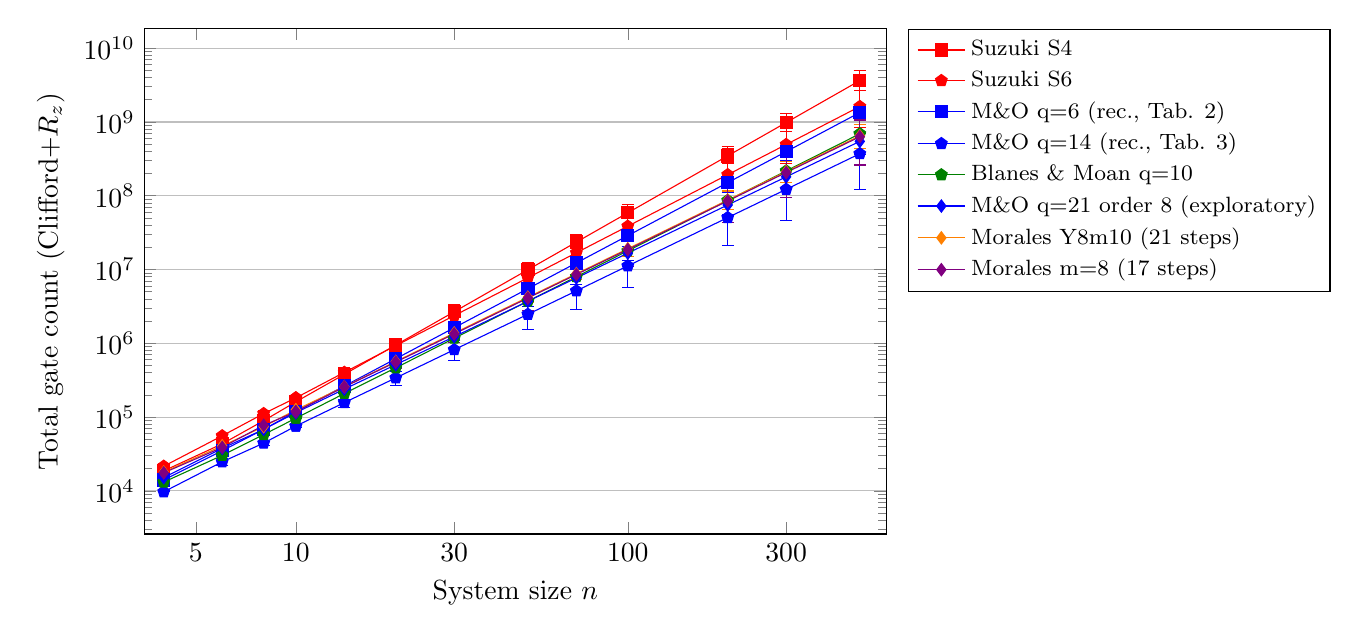
\begin{tikzpicture}
  \begin{loglogaxis}[
    width=11cm, height=8cm,
    xlabel={System size $n$},
    ylabel={Total gate count (Clifford+$R_z$)},
    xtick={5,10,30,100,300}, xticklabels={5,10,30,100,300},
    xmin=3.5, xmax=600,
    ymajorgrids=true,
    legend pos=outer north east,
    legend cell align=left,
    legend style={font=\footnotesize},
  ]
    % suzuki4: measured n, mean over seeds, bars min..max over seeds
    \addplot[red, solid, mark=square*, mark size=2.2pt, mark options={solid, fill=red}, error bars/.cd, y dir=both, y explicit, error bar style={solid}] coordinates {
      (4,18686.4) += (0,549.6) -= (0,366.4)
      (6,43418.4) += (0,549.6) -= (0,824.4)
      (8,89401.6) += (0,4030.4) -= (0,3297.6)
      (10,161102) += (0,6068.5) -= (0,5381.5)
    };
    \addlegendentry{Suzuki S4}
    % suzuki4: extrapolated, r = ceil(3.81587 n^1.56408), per step = 229/2 n + 0; bars min..max of per-seed fits
    \addplot[red, solid, mark=square*, mark size=2.2pt, mark options={solid, fill=red}, forget plot, error bars/.cd, y dir=both, y explicit, error bar style={solid}] coordinates {
      (10,161102)
      (14,379911) += (0,19236) -= (0,16030)
      (20,948060) += (0,73280) -= (0,61830)
      (30,2.6793e+06) += (0,291975) -= (0,247320)
      (50,9.92715e+06) += (0,1.49995e+06) -= (0,1.25378e+06)
      (70,2.3524e+07) += (0,4.21589e+06) -= (0,3.4705e+06)
      (100,5.86927e+07) += (0,1.23546e+07) -= (0,9.9386e+06)
      (200,3.47095e+08) += (0,9.47144e+07) -= (0,7.30052e+07)
      (300,9.8162e+08) += (0,3.05268e+08) -= (0,2.29046e+08)
      (500,3.63732e+09) += (0,1.31154e+09) -= (0,9.50636e+08)
    };
    % suzuki6: measured n, mean over seeds, bars min..max over seeds
    \addplot[red, solid, mark=pentagon*, mark size=2.2pt, mark options={solid, fill=red}, error bars/.cd, y dir=both, y explicit, error bar style={solid}] coordinates {
      (4,21593.8) += (0,1924.2) -= (0,213.8)
      (6,55801.8) += (0,1924.2) -= (0,4489.8)
      (8,111604) += (0,12400.4) -= (0,13255.6)
      (10,182264) += (0,10155.5) -= (0,5879.5)
    };
    \addlegendentry{Suzuki S6}
    % suzuki6: extrapolated, r = ceil(1.64274 n^1.32149), per step = 1069/2 n + 0; bars min..max of per-seed fits
    \addplot[red, solid, mark=pentagon*, mark size=2.2pt, mark options={solid, fill=red}, forget plot, error bars/.cd, y dir=both, y explicit, error bar style={solid}] coordinates {
      (10,182264)
      (14,404082) += (0,67347) -= (0,44898)
      (20,930030) += (0,245870) -= (0,160350)
      (30,2.37318e+06) += (0,994170) -= (0,513120)
      (50,7.72352e+06) += (0,4.89068e+06) -= (0,2.11128e+06)
      (70,1.68742e+07) += (0,1.33197e+07) -= (0,5.2381e+06)
      (100,3.86444e+07) += (0,3.7415e+07) -= (0,1.3416e+07)
      (200,1.92954e+08) += (0,2.65753e+08) -= (0,7.93198e+07)
      (300,4.94519e+08) += (0,8.17625e+08) -= (0,2.20642e+08)
      (500,1.61873e+09) += (0,3.31337e+09) -= (0,7.88922e+08)
    };
    % mo-q6: measured n, mean over seeds, bars min..max over seeds
    \addplot[blue, solid, mark=square*, mark size=2.2pt, mark options={solid, fill=blue}, error bars/.cd, y dir=both, y explicit, error bar style={solid}] coordinates {
      (4,14092) += (0,0) -= (0,0)
      (6,35040.3) += (0,731.7) -= (0,81.3)
      (8,68292) += (0,0) -= (0,0)
      (10,118834) += (0,1761.5) -= (0,2303.5)
    };
    \addlegendentry{M\&O q=6 (rec., Tab. 2)}
    % mo-q6: extrapolated, r = ceil(3.56738 n^1.38733), per step = 271/2 n + 0; bars min..max of per-seed fits
    \addplot[blue, solid, mark=square*, mark size=2.2pt, mark options={solid, fill=blue}, forget plot, error bars/.cd, y dir=both, y explicit, error bar style={solid}] coordinates {
      (10,118834)
      (14,263683) += (0,7588) -= (0,5691)
      (20,617880) += (0,21680) -= (0,21680)
      (30,1.626e+06) += (0,77235) -= (0,77235)
      (50,5.5013e+06) += (0,365850) -= (0,352300)
      (70,1.22831e+07) += (0,948500) -= (0,910560)
      (100,2.87802e+07) += (0,2.58805e+06) -= (0,2.439e+06)
      (200,1.5054e+08) += (0,1.72356e+07) -= (0,1.5718e+07)
      (300,3.96297e+08) += (0,5.11377e+07) -= (0,4.59345e+07)
      (500,1.34165e+09) += (0,1.98236e+08) -= (0,1.75066e+08)
    };
    % mo-q14: measured n, mean over seeds, bars min..max over seeds
    \addplot[blue, solid, mark=pentagon*, mark size=2.2pt, mark options={solid, fill=blue}, error bars/.cd, y dir=both, y explicit, error bar style={solid}] coordinates {
      (4,9712) += (0,0) -= (0,0)
      (6,24765.6) += (0,2549.4) -= (0,2913.6)
      (8,44432.4) += (0,1699.6) -= (0,3156.4)
      (10,75571.5) += (0,3338.5) -= (0,2731.5)
    };
    \addlegendentry{M\&O q=14 (rec., Tab. 3)}
    % mo-q14: extrapolated, r = ceil(1.63049 n^1.17678), per step = 607/2 n + 0; bars min..max of per-seed fits
    \addplot[blue, solid, mark=pentagon*, mark size=2.2pt, mark options={solid, fill=blue}, forget plot, error bars/.cd, y dir=both, y explicit, error bar style={solid}] coordinates {
      (10,75571.5)
      (14,157213) += (0,16996) -= (0,21245)
      (20,339920) += (0,72840) -= (0,72840)
      (30,819450) += (0,282255) -= (0,236730)
      (50,2.47352e+06) += (0,1.35058e+06) -= (0,940850)
      (70,5.14129e+06) += (0,3.52667e+06) -= (0,2.25197e+06)
      (100,1.11992e+07) += (0,9.43885e+06) -= (0,5.49335e+06)
      (200,5.05631e+07) += (0,6.10035e+07) -= (0,2.91967e+07)
      (300,1.22098e+08) += (0,1.77456e+08) -= (0,7.57536e+07)
      (500,3.7118e+08) += (0,6.68155e+08) -= (0,2.48566e+08)
    };
    % bm-q10: measured n, mean over seeds, bars min..max over seeds
    \addplot[green!50!black, solid, mark=pentagon*, mark size=2.2pt, mark options={solid, fill=green!50!black}, error bars/.cd, y dir=both, y explicit, error bar style={solid}] coordinates {
      (4,13170) += (0,0) -= (0,0)
      (6,30291) += (0,0) -= (0,0)
      (8,57948) += (0,0) -= (0,0)
      (10,96580) += (0,0) -= (0,0)
    };
    \addlegendentry{Blanes \& Moan q=10}
    % bm-q10: extrapolated, r = ceil(2.36355 n^1.26919), per step = 439/2 n + 0; bars min..max of per-seed fits
    \addplot[green!50!black, solid, mark=pentagon*, mark size=2.2pt, mark options={solid, fill=green!50!black}, forget plot, error bars/.cd, y dir=both, y explicit, error bar style={solid}] coordinates {
      (10,96580)
      (14,208964) += (0,0) -= (0,0)
      (20,465340) += (0,0) -= (0,0)
      (30,1.17213e+06) += (0,0) -= (0,0)
      (50,3.72052e+06) += (0,0) -= (0,0)
      (70,7.9898e+06) += (0,0) -= (0,0)
      (100,1.79332e+07) += (0,0) -= (0,0)
      (200,8.63952e+07) += (0,0) -= (0,0)
      (300,2.16844e+08) += (0,0) -= (0,0)
      (500,6.91096e+08) += (0,0) -= (0,0)
    };
    % mo-o8-q21: measured n, mean over seeds, bars min..max over seeds
    \addplot[blue, solid, mark=diamond*, mark size=2.2pt, mark options={solid, fill=blue}, error bars/.cd, y dir=both, y explicit, error bar style={solid}] coordinates {
      (4,15136.8) += (0,1081.2) -= (0,720.8)
      (6,37842) += (0,2703) -= (0,2703)
      (8,68115.6) += (0,3964.4) -= (0,3243.6)
      (10,114878) += (0,6757.5) -= (0,2252.5)
    };
    \addlegendentry{M\&O q=21 order 8 (exploratory)}
    % mo-o8-q21: extrapolated, r = ceil(1.70915 n^1.16766), per step = 901/2 n + 0; bars min..max of per-seed fits
    \addplot[blue, solid, mark=diamond*, mark size=2.2pt, mark options={solid, fill=blue}, forget plot, error bars/.cd, y dir=both, y explicit, error bar style={solid}] coordinates {
      (10,114878)
      (14,239666) += (0,31535) -= (0,12614)
      (20,513570) += (0,117130) -= (0,36040)
      (30,1.22986e+06) += (0,445995) -= (0,121635)
      (50,3.71662e+06) += (0,2.04978e+06) -= (0,540600)
      (70,7.69454e+06) += (0,5.29788e+06) -= (0,1.356e+06)
      (100,1.66685e+07) += (0,1.41006e+07) -= (0,3.4238e+06)
      (200,7.49632e+07) += (0,8.9199e+07) -= (0,1.95517e+07)
      (300,1.80425e+08) += (0,2.5692e+08) -= (0,5.25734e+07)
      (500,5.45781e+08) += (0,9.57087e+08) -= (0,1.78623e+08)
    };
    % morales-y8m10: measured n, mean over seeds, bars min..max over seeds
    \addplot[orange, solid, mark=diamond*, mark size=2.2pt, mark options={solid, fill=orange}, error bars/.cd, y dir=both, y explicit, error bar style={solid}] coordinates {
      (4,18020) += (0,0) -= (0,0)
      (6,40815.3) += (0,2432.7) -= (0,270.3)
      (8,74242.4) += (0,1441.6) -= (0,2162.4)
      (10,125239) += (0,5406) -= (0,3604)
    };
    \addlegendentry{Morales Y8m10 (21 steps)}
    % morales-y8m10: extrapolated, r = ceil(1.77538 n^1.18938), per step = 901/2 n + 0; bars min..max of per-seed fits
    \addplot[orange, solid, mark=diamond*, mark size=2.2pt, mark options={solid, fill=orange}, forget plot, error bars/.cd, y dir=both, y explicit, error bar style={solid}] coordinates {
      (10,125239)
      (14,258587) += (0,18921) -= (0,6307)
      (20,567630) += (0,54060) -= (0,36040)
      (30,1.37853e+06) += (0,175695) -= (0,135150)
      (50,4.21218e+06) += (0,743325) -= (0,630700)
      (70,8.76673e+06) += (0,1.8921e+06) -= (0,1.51368e+06)
      (100,1.91462e+07) += (0,4.82035e+06) -= (0,3.91935e+06)
      (200,8.73069e+07) += (0,2.8832e+07) -= (0,2.2525e+07)
      (300,2.1205e+08) += (0,8.02791e+07) -= (0,6.10878e+07)
      (500,6.4872e+08) += (0,2.86518e+08) -= (0,2.10158e+08)
    };
    % morales-m8: measured n, mean over seeds, bars min..max over seeds
    \addplot[violet, solid, mark=diamond*, mark size=2.2pt, mark options={solid, fill=violet}, error bars/.cd, y dir=both, y explicit, error bar style={solid}] coordinates {
      (4,17592) += (0,0) -= (0,0)
      (6,38922.3) += (0,2858.7) -= (0,1539.3)
      (8,77404.8) += (0,1759.2) -= (0,1172.8)
      (10,118380) += (0,2565.5) -= (0,4764.5)
    };
    \addlegendentry{Morales m=8 (17 steps)}
    % morales-m8: extrapolated, r = ceil(2.14576 n^1.18752), per step = 733/2 n + 0; bars min..max of per-seed fits
    \addplot[violet, solid, mark=diamond*, mark size=2.2pt, mark options={solid, fill=violet}, forget plot, error bars/.cd, y dir=both, y explicit, error bar style={solid}] coordinates {
      (10,118380)
      (14,256550) += (0,20524) -= (0,25655)
      (20,557080) += (0,65970) -= (0,95290)
      (30,1.34139e+06) += (0,252885) -= (0,318855)
      (50,4.1048e+06) += (0,1.08118e+06) -= (0,1.30108e+06)
      (70,8.56877e+06) += (0,2.71943e+06) -= (0,3.15556e+06)
      (100,1.86548e+07) += (0,7.07345e+06) -= (0,7.6965e+06)
      (200,8.5028e+07) += (0,4.28072e+07) -= (0,4.21475e+07)
      (300,2.06266e+08) += (0,1.20175e+08) -= (0,1.1094e+08)
      (500,6.30563e+08) += (0,4.33386e+08) -= (0,3.69798e+08)
    };
  \end{loglogaxis}
\end{tikzpicture}
